% !TEX root = MAIN.tex
\clearpage
\section{Test Suite Augmentation}
\label{sec:testGeneration}



\begin{figure}[tb]
\begin{center}
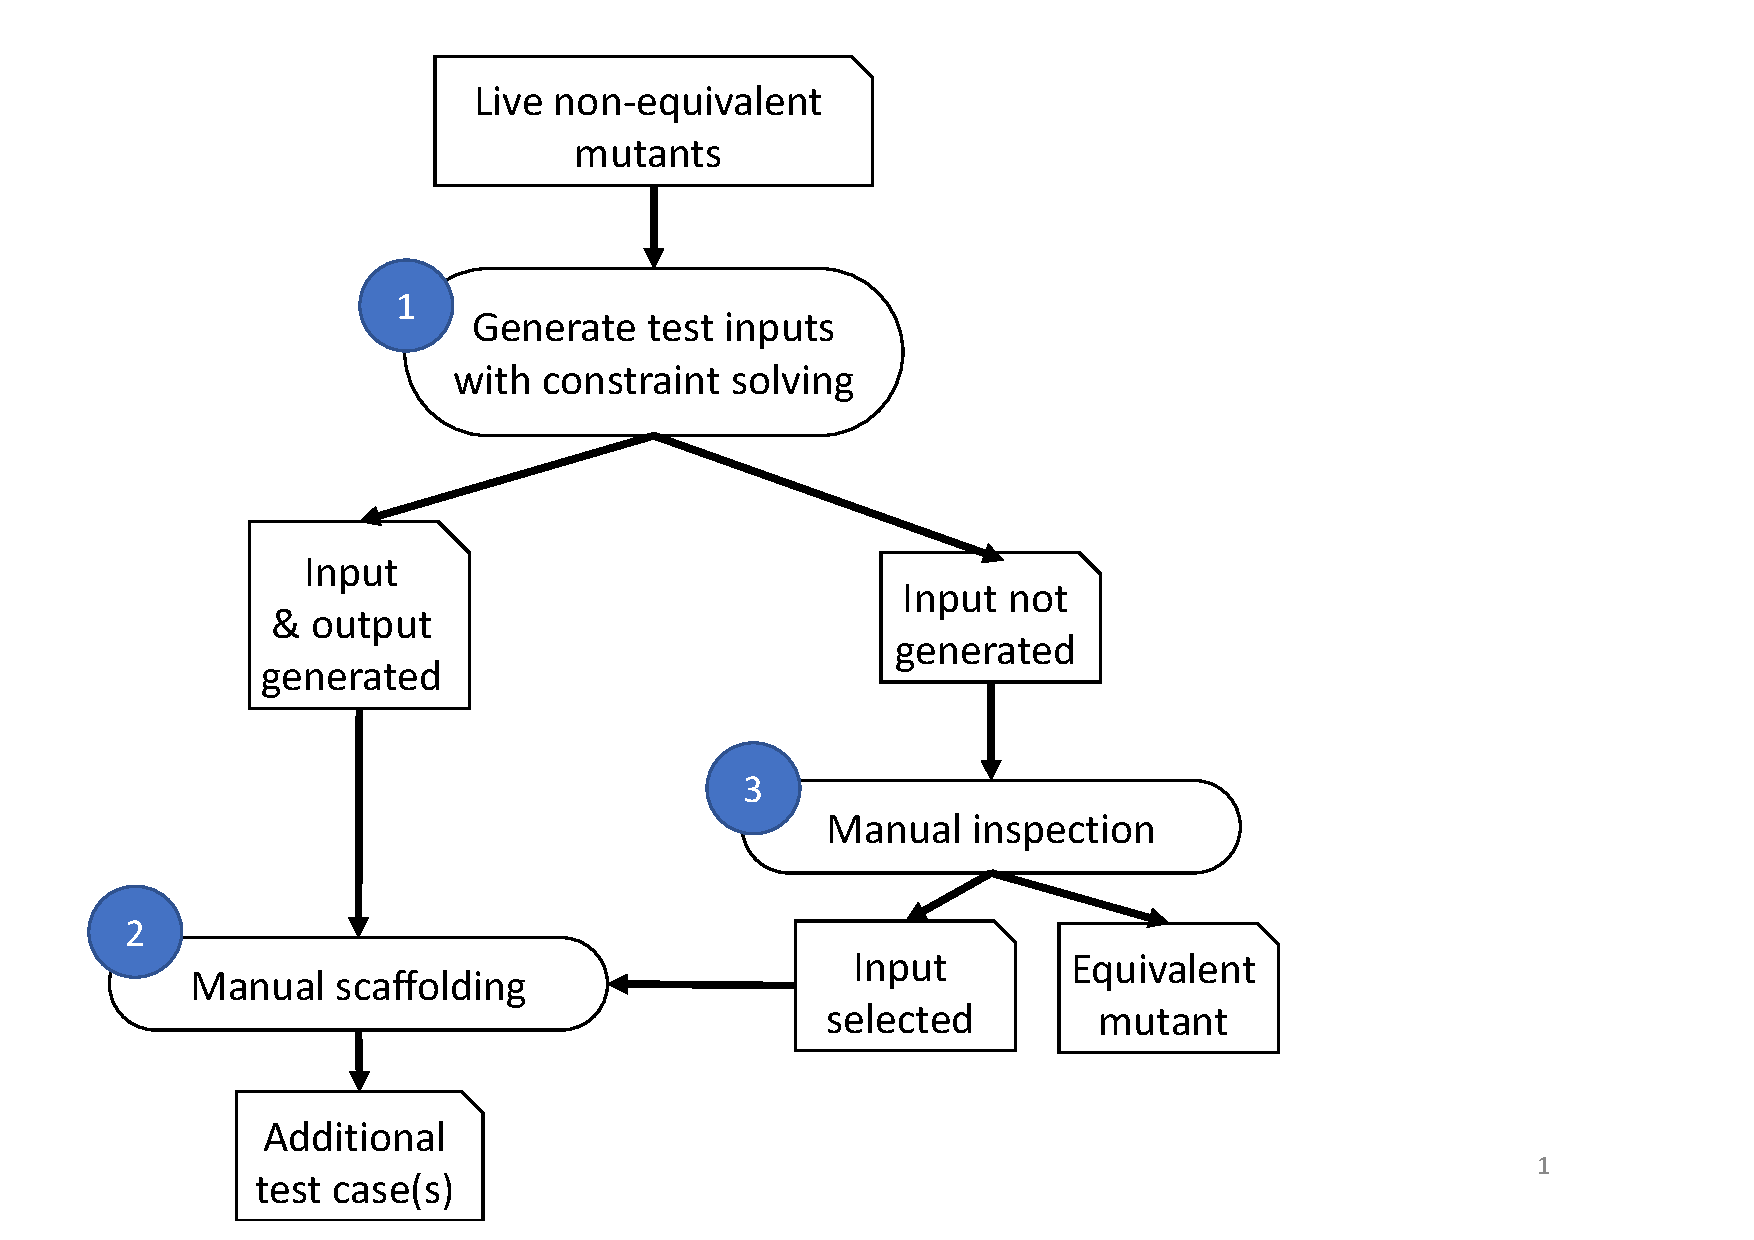
\includegraphics[width=8cm]{images/codeDrivenTestSuiteAugmentationProcess}
\caption{Overview of the proposed Test Suite Augmentation Process}
\label{fig:codeDrivenTestSuiteAugmentationProcess}
\end{center}
\end{figure}



%\TODO{This section still needs to be filled}
Figure~\ref{fig:codeDrivenTestSuiteAugmentationProcess} shows the test suite augmentation process for code-driven mutation testing. 
It aims to automatically generate unit tests for the functions with live mutants.

According to our process, each live, non-equivalent mutant identified by the test suite assessment process is analyzed by means of static analysis tools based on constraint-solving (Step 1). 

We leverage the approach proposed by Holling et al.~\cite{holling2016nequivack} and Riener et al.~\cite{riener2011test}, which  relies on the observation that two mutants are equivalent when there are no concrete values making the mutated function produce an output that is different from the one of the original function.
If a value that makes the two functions generate distinct results can be found, the mutant is non-equivalent.
To automate the generation of inputs, Holling et al. rely on KLEE~\cite{cadar2008klee}, a symbolic execution tool for programs written in C/C++.
Riener et al.~\cite{riener2011test}, instead, rely on a bounded model checker (BMC).

We introduce an example in Listing~\ref{function}. The top part of Listing~\ref{function} shows the function \texttt{isPositive}, which checks if an integer number is positive or not. The bottom part of Listing~\ref{function} presents the mutated version of \texttt{isPositive}, where the relational operator $\geq$ has been replaced by the operator $>$.
To automate the generation of inputs, static analysis tools need to be informed about which parameters correspond to inputs. 
In Listing~\ref{example}, this is achieved by function \texttt{make\_symbolic} which converts concrete variables to symbolic ones by considering their memory address and size (Line 3). 
%In Listing~\ref{example}, the parameter \texttt{numSymbolic} is made symbolic in Line 3. 
Then, the original and mutated functions are called using the same arguments (Lines 5 and 6).
Finally, we need an assertion indicating that the return values of the two functions the same (see Line 8).
Since the objective of static analysis tools is to look for inputs that falsify a given assertion, the provided assertion
will make the static analysis tools \EMPH{look for inputs that make the output of the two functions different}. 
%Despite being counter-intuitive, this approach is effective because symbolic execution engines aim to identify inputs that falsify the assertions in the program. 
When the equality is falsified, then the two functions can produce a different output for a same input.
The input that falsifies the equality can thus be used to improve the test suite enabling it to kill the mutant.
% make the original an mutate function geenrate distinct results
% of identifying inputs that lead to different output falsifying the assertion.

%In the concrete, if we consider the implementation of \texttt{isPositive} and \texttt{MUT\_isPositive}, 
In the example of Listing~\ref{example}, the static analysis tool will indicate that the return values of the original and mutated function differ when \texttt{num} is equal to zero.
A new test case exercising function \texttt{isPositive} with \texttt{num=0} should thus be added to the test suite in order to kill the mutant.

\begin{lstlisting}[style=CStyle, caption=isPositive and MUT\_isPositive functions, label=function]
int isPositive(int num){
	if (num >= 0){
		return 1;
	} else {
		return 0;
	}
}

int MUT_isPositive(int num){
	if (num > 0){
		return 1;
	} else {
		return 0;
	}
}

\end{lstlisting}

\begin{lstlisting}[style=CStyle, caption=Holling's approach for test case generation., label=example]
void test () { 
	int numSymbolic; 
	make_symbolic(&numSymbolic, sizeof(numSymbolic), "numSymbolic"); 
 	
 	int original_ret = isPositive(numSymbolic); 
	int transformed_ret = MUT_isPositive(numSymbolic); 
 
	assert(original_ret == transformed_ret); 
}
\end{lstlisting}



Static analysis tools enable the identification of inputs that lead to different outputs for the original and the mutated program.
%Consequently, they can also be used to determine the output expected for the original software.
Also, they can also determine if such inputs do not exist, which happens when two mutants are equivalent.
In some cases, static analysis tools may not be able to provide a result.
Mutants for which it is not possible to automatically identify a killing input needs to be manually inspected (Step 3).
 %(i.e., the outputs that distinguish the original software from the mutant). 
 
 The generated inputs and the identified outputs are used by the engineers who can manually implement a test case by reusing such inputs and outputs to define the inputs and the assertions for a test case that kills the mutant (Step 2).  The outputs simply reflect the behaviour of the program implementation, which might be faulty. For this reason, when writing oracles (E.g., assert statements) based on the provided outputs, engineers should very that the provided output is correct, based on the specifications of the software.
 


Step 1 is the only step that is automated by existing tools; anyway, it requires the manual specification of which are the inputs and the outputs of the function under test. In the project, two tools will be considered: CBMC, a bounded model checker, and KLEE~\cite{cadar2008klee}. The process to be automated in the two cases is defined in the following subsections.

\subsection{CBMC}
\label{subsec:cbmc}

CBMC is an approach that implements {\em Bounded Model
Checking}~\cite{BiereCCZ:TACAS99,SeryFS:ATVA12} (BMC), an approach for purely static software verification.
The idea in BMC is to represent the software together with the
properties to be verified as an instance of the propositional
satisfiability problem (SAT).  Such a representation captures the
software behavior exactly, assuming that all the loop bodies in the
software are repeated at most a fixed number of times.
%
This approach has several advantages: the logical formulation is usually
very compact compared to traditional model checking, where verification
is reduced to a reachability problem in a graph representing the program
state space;
%
there are several high-performance SAT
solvers~\cite{MarquesSilva:IEEETRAN99,EenS:SAT2003} that can be used for
solving the instances;
%
and the satisfying assignments of an instance can be directly translated
to meaningful counterexamples for correctness in the form of
fault-inducing executions.
%
Furthermore, it is widely recognized that BMC based approaches are particularly good
at quickly finding short counterexamples when they exist.

A {\em bounded model checker} takes as input a program $\prog$, a bound $k$
for loop unrolling, and a set $S$ of properties to be verified against
$\prog$, and returns for each property ${l}$ in $S$, expressed as a propositional statement over variables of $\prog$ at a location $l$, either \vspace{-0.2cm}
\begin{itemize}
    \item \emph{verified}, if the executions of $\prog$  satisfy $\prop{l}$;\vspace{-0.25cm}
    \item \emph{unreachable}, if no execution of $\prog$ reaches $l$;\vspace{-0.25cm}
    \item \emph{false}, if there is an execution of $\prog$
    where the property $l$ is broken; and\vspace{-0.25cm}
    \item \emph{unknown}, if the checker is unable, due to
    memory or time limits, to determine whether ${l}$ holds,\vspace{-0.2cm}
\end{itemize}
under the assumption that no loop body in the program is repeated more
than $k$ times.

The approach is naturally a compromise between practicality and
completeness.
As the SAT problem is NP-complete, determining whether $\prop{l}$ holds
requires in the worst case exponential time with respect to the size of
the SAT instance for all known algorithms.
%
Furthermore, the instances can in some cases grow very large since many
operations, such as multiplication, have quadratic encodings in SAT and,
for example, the instance grows exponentially in number of nested loops.
%

Due to numerous optimizations BMC can nevertheless solve many practical
problems in reasonable time and memory limits.
%
For example, the size of the resulting SAT instance can be dramatically
reduced by slicing off parts of the program that do not affect the
validity of the property being checked, and
%
extremely efficient SAT solver implementations which learn the instance
structure and use adaptive heuristics~\cite{MahajanFM:SAT04} rarely
suffer from the exponential worst-case behavior in problems emerging
from applications.
%
The fact that bounded model checkers only prove correctness of
properties for executions not exceeding the bound $k$ is also beneficial
in many ways for detecting regressions.  In addition to obvious
performance benefits our experiments show that in most cases even a single
loop iteration is sufficient to indicate a regression between two
versions, and a small bound guarantees in a natural way that the
reported counterexamples are short.

In the context of FAQAS, we aim to rely on BMC to automatically identify the inputs that make the mutated function generate an output different than the original function. This happens when the outcome of the verification is \emph{false}, i.e., the assertion indicating that the output of the original and mutate program are the same does not hold. In this case the BMC tool returns also a trace with the values of inputs and outputs for the two functions along with the assignment of all the program variables defined within a simulated program execution.

When the outcome of the verification is \emph{true}, the assertion indicating that the output of the original and mutate program are the same holds. This means that the the mutant is equivalent and thus can be ignored. In this case we suggest engineers to double heck the results because the mutant might be equivalent because of  the bound $k$.

When the outcome of the verification is \emph{unknown}, the engineer needs to manually inspect the source code to determine if the mutant is equivalent.

We do not envision cases where the outcome of the verification is \emph{unreachable}; indeed, since the assertion is manually introduced it should be reached.



% !TEX root =  ../MAIN.tex
\begin{minipage}{14cm}
\begin{lstlisting}[style=CStyle, caption=Example of code for the identification of inputs., label=GSLaugmentation]
/* Copyright (c) 2013-2017 GomSpace A/S. All rights reserved. */
  
#include <gs/util/byteorder.h>
#include <assert.h>

...

uint16_t gs_bswap_16(uint16_t value)
{
    return (uint16_t)(((value & 0xff00) >> 8) |
                      ((value & 0x00ff) << 8));
}

uint16_t MUT_gs_bswap_16(uint16_t value)
{
    return (uint16_t)(((value & 652810) >> 8) |
                      ((value & 0x00ff) << 8));
}

...

int main(){
        uint16_t v = nondet_uint16_t();
        uint16_t res;
        uint16_t resMUT;

        res = gs_bswap_16(v);
        resMUT = MUT_gs_bswap_16(v);

        __CPROVER_output("input: v", v);
        __CPROVER_output("output original: res", res);
        __CPROVER_output("output mutated: resMut", resMUT);

        assert( res == resMUT );
}
\end{lstlisting}
\end{minipage}


Listing~\ref{GSLaugmentation} shows an input file for CBMC that enables the automated identification of inputs to kill one mutant (\emph{MUT\_gs\_bswap\_16}) for function \emph{gs\_bswap\_16} belonging to GSL case study libUtils. The mutant 
is not killed by GSL test suite. Function \emph{cbmc\_main} is used to declare all the variables and assertions to be processed by CBMC to generate the required inputs for testing.

The command used to execute CBMC for this example is
\begin{verbatim}
cbmc -I include/ --property cbmc_main.assertion.1 --trace --function cbmc_main 
   --no-unwinding-assertions --unwind 5 src/byteorder.c
\end{verbatim}

Although CBMC can be integrated into build systems to process large code bases; to minimize the risk of encountering difficulties in parsing large projects, we believe the simplest solution consists of executing CBMC against the source file containing the mutated function. With such configuration, CBMC will ignore dependencies (i.e., functions invoked by the function under test) and threat them as generating random values. This will speed-up execution but may lead to wrong results due to randomness. One solution to minimize such wrong results is to first execute CBMC to prove that the function can deterministically return the same value, if it is the case, dependencies can be ignored. Otherwise these dependencies need to be included or assumptions about their output values (e.g., always positive) need to be specified using the functions provided by CBMC. Evaluation of the best configuration for CBMC should be an outcome of the project.

Engineers need to declare all the variables that correspond to inputs for the mutated function as \emph{nondet\_<type>}. Function \emph{\_\_CPROVER\_output} is used to print the values identified by the execution of CBMC.

Figure~\ref{fig:cbmcOutput} shows the output generated by CBMC when processing the function. It indicates that for the input \emph{v=2048}, the result obtained with the original program is the value \emph{8}, while for the mutated program it is the value \emph{0}. Listing~\ref{GSLaugmentationTest} shows a test case manually written based on the output produced by CBMC.

\begin{figure}[h]
\begin{center}
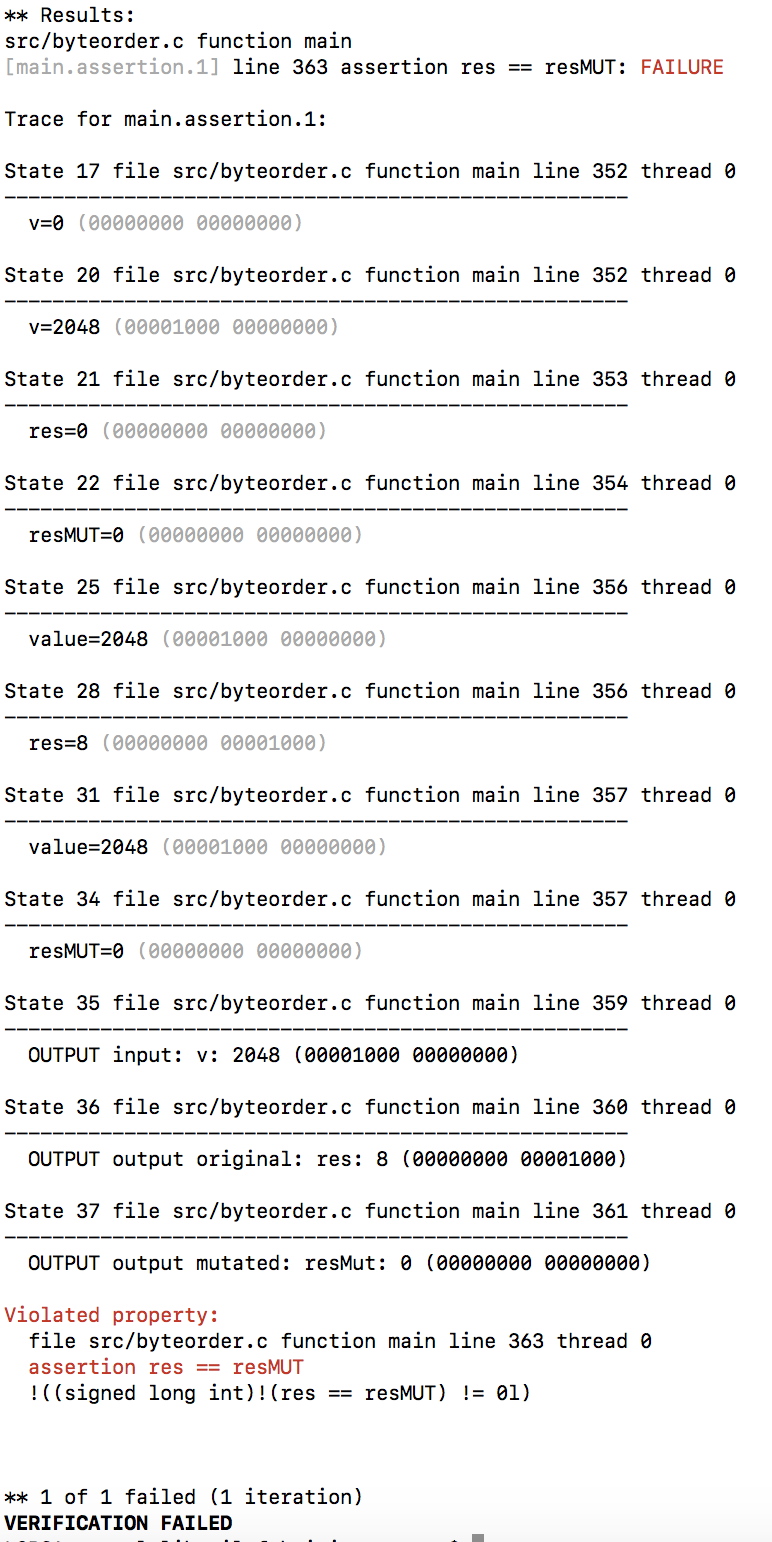
\includegraphics[width=8cm]{images/CBMCoutput}
\caption{CBMC output}
\label{fig:cbmcOutput}
\end{center}
\end{figure}

% !TEX root =  ../MAIN.tex
\begin{minipage}{14cm}
\begin{lstlisting}[style=CStyle, caption=Example of test case for function \emph{gs\_bswap\_16} derived from CBMC output., label=GSLaugmentationTest]
int main(){
        uint16_t v = 2048;
        uint16_t res;

        res = gs_bswap_16(v);

        assert( res == 8 );
        return 0;
}
\end{lstlisting}
\end{minipage}


\clearpage



Listing~\ref{GSLaugmentationTwo} shows another example of a source file to be parsed by CBMC to automatically derive inputs for a test case. Function \emph{cbmc\_main} provide the setup for CBMC. Function \emph{main} is the test case manually implemented after observing CBMC output. 
Listing~\ref{GSLaugmentationTwo} shows one of the main \INDEX{limitations of CBMC}, i.e., the fact that it requires some standard library functions to be redefined. Indeed, although CBMC includes a few definitions for standard library functions, some of them are generalizations (i.e., CBMC does not aim to replicate the actual behaviour but just to preserve high-level post-conditions) and the original source code of the implementation may need to be provided in order to obtain correct results.

% !TEX root =  ../MAIN.tex

\begin{lstlisting}[style=CStyle, caption=Second example of code for the identification of inputs with CBMC., label=GSLaugmentationTwo]
#include <gs/util/base16.h>
#include <stdio.h>
#include <stdlib.h>
#include <limits.h>
//The following should not be included, otherwise CBMC will lead to wrong results
//#include <ctype.h>
#include <errno.h>
#include <assert.h>


//The following function had been defined because CBMC has a builtin definition of some stdlib function, but the definition is too generic
// and leads to non-deterministic behaviours
unsigned long
strtoul(nptr, endptr, base)
	const char *nptr;
	char **endptr;
	int base;
{
	const char *s = nptr;
	unsigned long acc;
	int c;
	unsigned long cutoff;
	int neg = 0, any, cutlim;

	/*
	 * See strtol for comments as to the logic used.
	 */
	do {
		c = *s++;
	} while (isspace(c));
	if (c == '-') {
		neg = 1;
		c = *s++;
	} else if (c == '+')
		c = *s++;
	if ((base == 0 || base == 16) &&
	    c == '0' && (*s == 'x' || *s == 'X')) {
		c = s[1];
		s += 2;
		base = 16;
	}
	if (base == 0)
		base = c == '0' ? 8 : 10;
	cutoff = (unsigned long)ULONG_MAX / (unsigned long)base;
	cutlim = (unsigned long)ULONG_MAX % (unsigned long)base;
	for (acc = 0, any = 0;; c = *s++) {
		if (isdigit(c))
			c -= '0';
		else if (isalpha(c))
			c -= isupper(c) ? 'A' - 10 : 'a' - 10;
		else
			break;
		if (c >= base)
			break;
		if (any < 0 || acc > cutoff || ( acc == cutoff && c > cutlim) )
			any = -1;
		else {
			any = 1;
			acc *= base;
			acc += c;
		}
	}
	if (any < 0) {
		acc = ULONG_MAX;
		errno = ERANGE;
	} else if (neg)
		acc = -acc;
	if (endptr != 0)
		*endptr = (char *)(any ? s - 1 : nptr);
	return (acc);
}



void base16_encode(const uint8_t * raw, size_t len, char *encoded)
{
        const uint8_t *raw_bytes = raw;
	char *encoded_bytes = encoded;
	size_t remaining = len;

	for (; remaining--; encoded_bytes += 2)
		snprintf(encoded_bytes, 3, "%02X", *(raw_bytes++));

}

int base16_decode(const char *encoded, uint8_t *raw)
{
    uint8_t *raw_bytes = raw;
    if (encoded) {
        const char *encoded_bytes = encoded;
        char buf[3];
        char *endp;

	while (encoded_bytes[0]) {
            if (!encoded_bytes[1]) {
                return GS_ERROR_ARG;
            }
            memcpy(buf, encoded_bytes, 2);
            buf[2] = '\0';
            *(raw_bytes++) = (uint8_t) strtoul(buf, &endp, 16);
            if (*endp != '\0') {
                return GS_ERROR_ARG;
            }
            encoded_bytes += 2;
	}
    }
    return (int)(raw_bytes - raw);
}

int MUT_base16_decode(const char *encoded, uint8_t *raw)
{
    uint8_t *raw_bytes = raw;
    if (encoded) {
        const char *encoded_bytes = encoded;
        char buf[3];
        char *endp;

	while (encoded_bytes[0]) {
            if (!encoded_bytes[1]) {
                //return GS_ERROR_ARG;
            }
            memcpy(buf, encoded_bytes, 2);
            buf[2] = '\0';
            *(raw_bytes++) = (uint8_t) strtoul(buf, &endp, 16);
            if (*endp != '\0') {
                return GS_ERROR_ARG;
            }
            encoded_bytes += 2;
	}
    }
    return (int)(raw_bytes - raw);
}


#ifdef CBMC
int cbmc_main(){
    char encoded[4];
	char a = nondet_char();
	char b = nondet_char();
	char c = nondet_char();

	uint8_t raw;
	uint8_t mRaw;
	int ret;
	int mret;

    
	encoded[0]=a;
	encoded[1]=b;
	encoded[2]=c;
    encoded[3]=0;

	raw=0;
    ret = base16_decode(encoded,&raw);

	encoded[0]=a;
	encoded[1]=b;
	encoded[2]=c;
        encoded[3]=0;
	mRaw=0;
    mret = MUT_base16_decode(encoded,&mRaw);
    
    //to verify that the original function is deterministic, just replace with the following
    //mret = base16_decode(encoded,&mRaw);


	__CPROVER_output("input: encoded", encoded);
	__CPROVER_output("output original: ret", ret);
	__CPROVER_output("output original: mret", mret);
	assert( ret == mret );
        
}
#endif

int main(){
    char encoded[4];

	uint8_t raw;
	uint8_t mRaw;
	int ret;
	int mret;

    
	encoded[0]='A';
	encoded[1]='D';
	encoded[2]='D';
    encoded[3]=0;

    ret = base16_decode(encoded,&raw);
    //ret = MUT_base16_decode(encoded,&raw);

	assert( ret == GS_ERROR_ARG );

    return 0;
}
\end{lstlisting}



% !TEX root = MAIN.tex

\subsection{KLEE}

KLEE is an approach that implements {\em Concolic Execution}, an approach that mixes concrete and symbolic execution.

...

In the context of FAQAS, we aim to rely on KLEE to automatically produce the inputs that make the mutated version of the program generate a different output than the original version.
This is observed in the outcome of the verification \emph{true}, i.e., the assertion indicating that the output of the original and mutated program are different does hold. In this case, KLEE produces the values of the inputs for which both versions of the program have a different result.

When the outcome of the verification is \emph{false}, the assertion that indicates if the output of the original and mutated program are the same does not hold. A \emph{false} outcome means that the mutant is equivalent and thus the test case can be ignored. 
We only consider the test inputs produced when the verification of the assertion holds.

% !TEX root =  ../MAIN.tex
\begin{minipage}{14cm}
\begin{lstlisting}[style=CStyle, caption=Example of code for the identification of inputs with KLEE., label=GSLaugmentation_klee]
/* Copyright (c) 2013-2017 GomSpace A/S. All rights reserved. */
  
#include <gs/util/byteorder.h>
#include <assert.h>

...

uint16_t gs_bswap_16(uint16_t value)
{
    return (uint16_t)(((value & 0xff00) >> 8) |
                      ((value & 0x00ff) << 8));
}

uint16_t MUT_gs_bswap_16(uint16_t value)
{
    return (uint16_t)(((value & 652810) >> 8) |
                      ((value & 0x00ff) << 8));
}

...

int main()
{
    uint16_t valueSymbolic;
    klee_make_symbolic(&valueSymbolic, sizeof(valueSymbolic), "valueSymbolic");

    uint16_t res = gs_bswap_16(valueSymbolic);
    uint16_t resMUT = MUT_gs_bswap_16(valueSymbolic);

    assert(res != resMUT);
    
    printf ("res %u resMUT %u\n", res, resMUT);
} 
\end{lstlisting}
\end{minipage}


Listing~\ref{GSLaugmentation_klee} shows an example of generation of inputs with KLEE for the mutant \linebreak\emph{MUT\_gs\_bswap\_16} presented in Listing~\ref{GSLaugmentation}. In this case, the function \emph{main} is used to declare all the variables and assertions to be processed by KLEE to generate the required inputs for testing. Particularly, the function creates an input of type \texttt{uint16\_t} with a symbolic value given by the KLEE function \texttt{klee\_make\_symbolic}. The symbolic value is then passed to both the original and the mutated functions. To produce test inputs that kill mutants the assertion of line 30 should be inserted.

To run this example, the program must be compiled with clang, instead of its original compiler, and with the \texttt{-emit-llvm} option enabled, since KLEE runs on bitcode rather than source code or binaries. The command used to compile this example is the following:

\begin{verbatim}
clang -DKLEE -I ~/klee/include -Iinclude -emit-llvm -c -g -O0 -Xclang 
-disable-O0-optnone byteorder.c
\end{verbatim}

By default, KLEE works on programs that do not use any external code such as C library functions. To enable KLEE to work with external code the KLEE POSIX runtime capability should be enabled. To generate the test inputs for this example, the following command should be used:

\begin{verbatim}
~/klee/build/bin/klee --libc=uclibc --posix-runtime byteorder.bc
\end{verbatim}

\begin{figure}[h]
\begin{center}
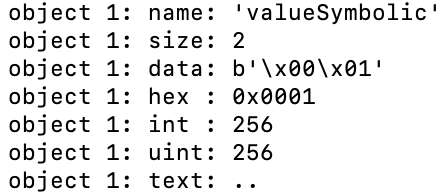
\includegraphics[width=0.4\textwidth]{images/klee_output_1}
\caption{KLEE output}
\label{fig:klee_output_1}
\end{center}
\end{figure}

% !TEX root =  ../MAIN.tex
\begin{minipage}{14cm}
\begin{lstlisting}[style=CStyle, caption=Example of test case for function \emph{gs\_bswap\_16} derived from KLEE output., label=GSLaugmentationTest_klee]
int main(){
    uint16_t v = 256;                                                                                                                                  
    uint16_t res;
    uint16_t resMUT;

    res = gs_bswap_16(v);
    resMUT = MUT_gs_bswap_16(v);

    assert( res == resMUT );
    return 0;
}
\end{lstlisting}
\end{minipage}


Figure~\ref{fig:klee_output_1} shows the output generated by KLEE when processing the function. It indicates that for the input \emph{symbolicValue=256}, the outcome of the assertion \texttt{res != resMUT} holds. Listing~\ref{GSLaugmentationTest_klee} shows a test case manually written based on the output produced by KLEE.

% !TEX root =  ../MAIN.tex

\begin{lstlisting}[style=CStyle, caption=Second example of code for the identification of inputs with KLEE., label=GSLaugmentationTwo_klee]
#include <klee/klee.h>

#include <gs/util/base16.h>
#include <stdio.h>
#include <stdlib.h>
#include <limits.h>
#include <ctype.h>
#include <errno.h>
#include <assert.h>


int base16_decode(const char *encoded, uint8_t *raw)
{
    uint8_t *raw_bytes = raw;
    if (encoded) {
        const char *encoded_bytes = encoded;
        char buf[3];
        char *endp;

    while (encoded_bytes[0]) {
            if (!encoded_bytes[1]) {
                return GS_ERROR_ARG;
            }
            memcpy(buf, encoded_bytes, 2);
            buf[2] = '\0';
            *(raw_bytes++) = (uint8_t) strtoul(buf, &endp, 16);
            if (*endp != '\0') {
                return GS_ERROR_ARG;
            }
            encoded_bytes += 2;
    }
    }
    return (int)(raw_bytes - raw);
}

int MUT_base16_decode(const char *encoded, uint8_t *raw)
{
    uint8_t *raw_bytes = raw;
    if (encoded) {
        const char *encoded_bytes = encoded;
        char buf[3];
        char *endp;

    while (encoded_bytes[0]) {
            if (!encoded_bytes[1]) {
                //return GS_ERROR_ARG;
            }
            memcpy(buf, encoded_bytes, 2);
            buf[2] = '\0';
            *(raw_bytes++) = (uint8_t) strtoul(buf, &endp, 16);
            if (*endp != '\0') {
                return GS_ERROR_ARG;
            }
            encoded_bytes += 2;
    }
    }
    return (int)(raw_bytes - raw);
}


#ifdef KLEE
int main() 
{
    char encoded[4];
    char a,b,c;
    klee_make_symbolic(&a, sizeof(a), "a");
    klee_make_symbolic(&b, sizeof(b), "b");
    klee_make_symbolic(&c, sizeof(c), "c");
    uint8_t raw;
    uint8_t mRaw;
    int ret;
    int mret;

    
    encoded[0]=a;
    encoded[1]=b;
    encoded[2]=c;
    encoded[3]=0;

    raw=0;
    ret = base16_decode(encoded,&raw);

    encoded[0]=a;
    encoded[1]=b;
    encoded[2]=c;
    encoded[3]=0;

    mRaw=0;
    mret = MUT_base16_decode(encoded,&mRaw);
    printf ("ret %d mret %d\n", ret, mret);

    assert( ret != mret );
} 
#endif
\end{lstlisting}
\begin{lstlisting}[style=CStyle, caption=Test case derived for the example in Listing~\ref{GSLaugmentationTwo_klee}., label=GSLaugmentationTwo_kleeTest]
int main(){
    char encoded[4];

    uint8_t raw;
    int ret;

    encoded[0]=48;
    encoded[1]=0;
    encoded[2]=0;
    encoded[3]=0;

    raw=0;
    ret = base16_decode(encoded,&raw);


    assert( ret == GS_ERROR_ARG );
    return 0;
}
\end{lstlisting}



Listing~\ref{GSLaugmentationTwo_klee} shows another example of a source file to be parsed by KLEE to automatically derive inputs for a test case. Similar to Section~\ref{subsec:cbmc}, we also apply KLEE to the mutant \texttt{MUT\_base16\_decode}. Function \emph{main} provide the setup for KLEE. While function \emph{main} is the test case manually derived from the KLEE output.

Comparing Listings~\ref{GSLaugmentationTwo} and~\ref{GSLaugmentationTwo_klee} can be seen the advantages of KLEE; basically, is it not longer necessary to provide KLEE the implementation of standard library functions (e.g., \emph{strtoul}), because they are provided by the POSIX runtime capability. This capability makes easier the integration of KLEE with the case study systems of FAQAS, and makes the results more accurate, since KLEE is aware of the standard library functions definitions and implementations.



